\chapter{Modelos de Distribución de Probabilidad}
\section{Distribuciones Discretas}
\subsection{Distribución de Bernoulli}
Si la probabilidad de que ocurra un evento $p$ y la probabilidad de que no ocurra es $q(q=1-p)$, entonces se dice que la \textbf{v.a.} discreta $X$ se distribuye según Bernoulli, cuya función de cuantía está dada por:
$$p(x)=f(x)=P(X=x)=
\begin{cases}
p^x\cdot (1-p)^{1-x} &; x=0;1 \\
0 &; \text{otro caso}
\end{cases}
$$
Y cuya función de distribución acumulada es:
$$
F(X)=P(X=x)=
\begin{cases}
0 &; x<0\\
q=1-p &; 0\leq x < 1\\
1 &; x\geq 1
\end{cases}
$$

$$
X \sim Ber(x;p)\Rightarrow 
\begin{cases}
E(x)=\mu = p \\
V(x)=\sigma^2 = p\cdot q \\
D(x) = \sigma = \sqrt{p\cdot q}
\end{cases}
$$
Conocida como prueba o ensayo de Bernoulli, es un experimento que solo tiene 2 resultados posibles, a los cuales se los llama:
\begin{itemize}
\item Éxito $(p)$
\item Fracaso $(q)$
\end{itemize}
\subsection{Distribución Binomial}
Una \textbf{v.a.} discreta $X$ tiene distribución lineal si su función de cuantía está dada por:
$$
f(x)=
\begin{cases}
\displaystyle\binom{n}{x} p^x \cdot q^{n-x} &; x=0,1,2,\ldots,n \\
0 &; \text{otro caso}
\end{cases}
$$
Donde:
\begin{itemize}
\item $p:$ Probabilidad de éxito.
\item $n:$ Número de ensayo.
\item $x:$ Número de éxitos.
\end{itemize}
Las Funciones de Distribución Acumulada Binomialmente está definida por:
$$
F(x)=P(X\leq x)=
\begin{cases}
0 &; x<0 \\
\displaystyle\sum_{k=0}^{[\![ x ]\!]}\displaystyle\binom{n}{k} p^k q^{n-k} &; 0\leq x < n \\
1 &; x\geq n
\end{cases}
$$
$$
X \sim b(x;n,p)\Rightarrow 
\begin{cases}
E(x)=\mu = n\cdot p \\
V(x)=\sigma^2 = n\cdot p \cdot q \\
D(x)=\sigma=\sqrt{n\cdot p\cdot q}
\end{cases}
$$

\subsubsection{Características de la Distribución Binomial}
\begin{enumerate}
\item Se realiza $n$ pruebas , cada una independiente.
\item $p$ es la probabilidad de éxito en cada prueba que ocurra en un evento y se mantiene constante a travez de las $n$ pruebas.
\item El experimento es con reposición (sustitución por reemplazo).
\item Se da el valor de la \textbf{v.a.} $X$. La variación de $x$ es desde 0 hasta $n$.

\end{enumerate}

\subsubsection{Observaciones}
$$f(x)=b(x;n,p) \hspace{1cm} n \text{ y } p \text{ son parámetros.}$$
\subsubsection{Manejo de la Tabla Binomial}
\begin{enumerate}
\item $\displaystyle\binom{p\leq 0.50}{n\leq 20}\Rightarrow
b(x;n,p)=B(x;n,p)-B(x-1;n,p)
$
\item $\displaystyle\binom{p>0.50}{n\geq 20}\Rightarrow 
\begin{cases}
\textbf{(i.) }b(x;n,p)= B(n-x;n,1-p)-B(n-x-1;n,1-p) \\
\textbf{(ii.) }b(x;n,p)=b(n-x;n,1-p) \text{ luego de usar \textbf{(i.)}} \\
\textbf{(iii.) } B(x;n,p) = 1 - B(n-x-1;n,1-p)
\end{cases}
$
\end{enumerate}
\subsection{Distribución de Poisson}
Una \textbf{v.a.} discreta $X$ tiene distribución de Poisson, si su función de cuantía está dada por:
$$
p(x)=f(x)=
\begin{cases}
\dfrac{e^{-\lambda}\cdot \lambda^x}{x!};& x=0,1,2,\ldots \\
0 ;& \text{otro caso}
\end{cases}
$$
Parámetro: $\lambda > 0$  \\$ { } $\\
La distribución de Poisson se obtiene de 2 maneras:
\begin{enumerate}
\item $\lim_{\substack{ n\to \infty \\ p\to 0 }} \displaystyle\binom{n}{x}\cdot p^x \cdot q^{n-x}\backsimeq \dfrac{e^{-\lambda}\cdot \lambda^x}{x!} \hspace{1cm} x=0,1,2,\ldots$
\item $p(x)=f(x)=\dfrac{e^{-\lambda\cdot t}(\lambda\cdot t)^x}{x!} \hspace{1cm} x=0,1,2,\ldots$
\end{enumerate}
donde $t$ es la cantidad de medida (intervalo de tiempo, longitud, área, etc...) La \textbf{F.D.A.} de Poisson está dada por:
$$
F(x)=
\begin{cases}
0 &; x<0 \\
\displaystyle\sum_{k=0}^{[\![ x ]\!]} \dfrac{e^{-\lambda}\cdot \lambda^x}{x!} &; x\geq 0
\end{cases}
$$
$$
X \sim Poisson(x;\lambda)\Rightarrow
\begin{cases}
E(x) = \mu = \lambda = n\cdot p \\
V(x) = \sigma^2 = n\cdot p \\
D(x) = \sigma = \sqrt{\lambda}

\end{cases}
$$
\subsection{Distribución Geométrica}
También llamada Distribución de Pascal, es un modelo útil para aquellos procesos en los que se repiten pruebas hasta llegar al éxito o a un resultado deseado y tiene interesantes aplicaciones en los muestreos realizados de esta manera. Su función de cuantía está dada por:
$$
p(x)=f(x)=(1-p)^x\cdot p \hspace{1cm}x=0,1,2,\ldots \hspace{0.5cm};\hspace{0.5cm} (0<p<1)
$$
También implica la existencia de una dicotomía de posibles resultados y la independencia de las pruebas entre sí.
\subsubsection{Características de la Distribución Geométrica}
\begin{enumerate}
\item El proceso consta de un número no definido de pruebas o experimentos separados o separables. El proceso concluirá cuando se obtenga por primera vez el resultado deseado (éxito).

\item Cada prueba puede dar dos resultados mutuamente excluyentes : $A$ y no $A$

\item La probabilidad de obtener un resultado A en cada prueba es p y la de obtener un resultado no $A$ es $q$
siendo $(p + q = 1)$.
\end{enumerate}
La \textbf{F.D.A.} de esta distribución es:
$$
F(x)=
\begin{cases}
0 &;x<0 \\
\displaystyle\sum_{k=0}^{[\![ x ]\!]} (1-p)^k p  &; x\geq 0
\end{cases}
$$
Y se notará de la siguiente manera:
$$
X\sim G(p)\Rightarrow
\begin{cases}
E(x)=\mu= \dfrac{1}{p} \\ \vspace{0.01cm} \\
V(x)=\sigma^2 = \dfrac{1-p}{p^2}\\ \vspace{0.01cm} \\
D(x)=\sigma= \dfrac{\sqrt{1-p}}{p}
\end{cases}
$$
\subsection{Distribución Binomial Negativa}
Consideremos ahora un experimento aleatorio consistente en repeticiones independientes de
ensayos de Bernoulli con probabilidad de éxito constante, hasta que aparezca el éxito k-ésimo.
Es decir, en lugar de fijar el número de ensayos y observar el número de éxitos en esas n
realizaciones, se repiten las realizaciones hasta obtener un número determinado de éxitos y contabilizamos los fracasos. Definimos la variable aleatoria con
distribución binomial negativa
como aquella que modeliza el número de fracasos antes de que aparezca el éxito k-ésimo.
$$
p(x)=f(x)=\binom{x+\lambda-1}{x} (1-p)^x p^\lambda
$$
Su \textbf{F.D.A.} está dada por:
$$
F(x)=
\begin{cases}
0 &; x<0 \\
\displaystyle\sum_{k=0}^{[\![ x ]\!]} \binom{k+\lambda-1}{x} (1-p)^k p^\lambda &; x\geq 0
\end{cases}
$$
Denotada por:
$$
X\sim BN(\lambda,p)\Rightarrow
\begin{cases}
E(x)=\mu= \dfrac{\lambda(1-p)}{p} \\ \vspace{0.01cm} \\
V(x)=\sigma^2 = \dfrac{\lambda (1-p)}{p^2}\\ \vspace{0.01cm} \\
D(x)=\sigma= \dfrac{\sqrt{\lambda (1-p)}}{p}
\end{cases}
$$
\section{Distribuciones Continuas}
\subsection{Distribución Uniforme o Rectangular}
Se dice que una \textbf{v.a.} continua $X$ tiene distribución uniforme en el intervalo $[a,b]$, si su función de densidad está dada por:
$$
f(x) = 
\begin{cases}
\dfrac{1}{b-a} ;& a\leq x \leq b \\
0 ;& \text{en otro caso.}
\end{cases}
$$
Parámetros: $a,b$ \\$ { } $\\
La gráfica de esta función se muestra en la siguiente figura:
%PENDIENTE
La \textbf{F.D.A.} de $X$, distribuida uniformemente, está dada por:
$$
F(x)=P(X\leq x)=
\begin{cases}
0 ;& x<a \\
\displaystyle\int_{-\infty}^{x} \dfrac{1}{b-a} dx=\dfrac{x-a}{b-a} ;& a\leq x < b \\
1 ;& x\geq b
\end{cases}
$$ 
La gráfica de $F$ es:
%PENDIENTE
$$
X \sim U(x;a,b)\Rightarrow 
\begin{cases}
E(x)=\mu = \dfrac{a+b}{2} \\
V(x)=\sigma^2 = \dfrac{(b-a)^2}{12} \\
D(x)=\sigma = \dfrac{(b-a)\sqrt{3}}{6}
\end{cases}
$$
\subsection{Distribución Exponencial}
Sea $X$ una \textbf{v.a.} continua. Se dice que $X$ tiene distribución exponencial con el parámetro real $\lambda$, si su función de densidad está dada por:
$$
f(x)=
\begin{cases}
\lambda\cdot e^{-\lambda\cdot x} ,& x\geq 0 \\
0 ,& \text{en otro caso}
\end{cases}
$$
Parámetro: $\lambda>0$ \\${ }$\\
La gráfica de $f$, se muestra en la siguiente figura:

%TODO

La \textbf{F.D.A.} de $X$, distribuida exponencialmente está dada por:
$$
F(x)=P(X\leq x)=
\begin{cases}
0, & x<0 \\
\displaystyle\int_{-\infty}^{x} \lambda\cdot e^{-\lambda\cdot x} dx = 1-e^{-\lambda\cdot x} ,& x\geq 0
\end{cases}
$$
La gráfica de $F$, es la siguiente:
%PENDIENTE
$$
X\sim exp(x;\lambda)\Rightarrow
\begin{cases}
E(x) = \mu = \frac{1}{\lambda} \\
V(x) = \sigma^2 = \frac{1}{\lambda^2} \\
D(x) = \sigma = \frac{1}{\lambda}
\end{cases}
$$
\subsubsection{Propiedad Amnésica}
$$P(X>s+t / x> s)=P(X>t)$$

%REALIZAR TABLA DE DATOS DE LAS DISTRIBUCIONES, NO OLVIDAR
\subsection{Distribución Normal}
Una \textbf{v.a.} continua $X$ tiene distribución normal con media $E(x)=\mu \in \mathbb{R}$ y varianza $V(x)=\sigma^2 >0$, si su función de densidad está dada por:
$$
f(x) = N(x;\mu,\sigma^2)=N(\mu,\sigma^2)=\dfrac{1}{\sigma \cdot \sqrt{2\pi}}e^{-\frac{1}{2}(\frac{x-\mu}{\sigma})}, x\in \mathbb{R}
$$
La gráfica de $f(x)$ es la siguiente:
%PENDIENTE
\subsubsection{Características de la Curva Normal}
\begin{enumerate}
\item $f'(x)=0\Leftrightarrow x=\mu$
\item $x<\mu \Rightarrow f'(x)>0;$ luego $f$ es creciente en $]-\infty,\mu]$
\item $x>\mu \Rightarrow f'(x)<0;$ luego $f$ es decreciente en $[\mu,+\infty[$
\item La curva tiene un máximo en $x=\mu$. (Moda en $\mu$)
\item $f''(x)=0 \Leftrightarrow x = \mu + \sigma$
\item Los puntos de inflexión están en: $x=\mu-\sigma$ y $x=\mu+\sigma$.
\item La curva de la distribución normal es simétrica respecto de $\mu$.
\item La media, mediana y moda son iguales (coinciden).
\item El área total bajo la curva normal y arriba del eje horizontal, es igual a 1.
\item La curva de la distribución normal se extiende $]-\infty,+\infty[$.
\end{enumerate}
\subsubsection{Distribución Normal Estándar}
\subsection{Distribución Chi Cuadrado}
\subsection{Distribución T-Student}
\subsection{Distribución F (Fisher-Snedecor)}
Una v.a. contínua $X$ tiene distribución $F$, con $r_1$ grados de libertad en el numerador y $r_2$ grados de libertad en el denominador y se representa por:
$$ X \sim F(r_1,r_2) $$
Si su función de densidad está definida por:

$$
f(z)=
\begin{cases}
\dfrac{\Big(\dfrac{r_1}{r_2}\Big)^{\frac{r_1}{2}}\Gamma\Big(\dfrac{r_1+r_2}{2}\Big) }{\Gamma\Big(\dfrac{r_1}{2}\Big)\Gamma\Big(\dfrac{r_2}{2}\Big)}\cdot \dfrac{x^{\frac{r_1}{2}-1}}{\Big(1+\dfrac{r_1}{r_2}x\Big)^{\frac{r_1+r_2}{2}}} &;x>0 \\
0 &;\text{otro caso}
\end{cases}
$$

La siguiente figura muestra una curva particular de $F$, para valores particulares de $r_1,r_2$:
\begin{center}

\begin{tikzpicture}[
    declare function={
            gamma(\z)=2.506628274631*sqrt(1/\z)+ 0.20888568*(1/\z)^(1.5)+ 0.00870357*(1/\z)^(2.5)- (174.2106599*(1/\z)^(3.5))/25920- (715.6423511*(1/\z)^(4.5))/1244160)*exp((-ln(1/\z)-1)*\z;
        },
        declare function={
            beta(\x,\y)=gamma(\x)*gamma(\y)/gamma(\x+\y);
        },
    declare function={
        fdst(\x,\a,\b) = 1 / beta(\a/2, \b/2) * (\a/\b)^(\a/2) * \x^(\a/2-1) * (1 + \a/\b*\x)^(-(\a + \b)/2);
    }
]

\begin{axis}[
  no markers, domain=0:4, samples=300,
  axis lines*=left, xlabel=$x$, ylabel=$f(x)$,
  every axis y label/.style={at=(current axis.above origin),anchor=south},
  every axis x label/.style={at=(current axis.right of origin),anchor=west},
  height=5cm, width=12cm,
  xtick=\empty, ytick=\empty,
  enlargelimits=false, clip=false, axis on top,
  grid = major
  ]

\addplot [very thick,line width=0.3mm] {fdst(x,5,2)};

\end{axis}
\end{tikzpicture}
\end{center}


\subsubsection{Teorema}
Si $U$ y $V$ son v.a. independientes, tales que $U\sim \chi^2(r_1)$ y $V\sim\chi^2(r_2)$ entonces:
$$ X = \dfrac{\dfrac{U}{r_1}}{\dfrac{V}{r_2}}\sim F(r_1,r_2) $$
\subsubsection{Corolario}

$$
X\sim F(r_1,r_2)\Rightarrow
\begin{cases}
E(x)=\mu=\dfrac{r_2}{r_2-2} & \forall r_2>2 \\\vspace{0.05cm} \\
V(x)=\sigma^2=\dfrac{2r^2(r_1+r_2-2)}{r_2(r_2-2)^2(r_2-4)} & \forall r_2>4
\end{cases}
$$

\subsubsection{$\bigstar$ Manejo de la Tabla:}

Si $X\sim F(r_1,r_2)$, entonces en la tabla de probabilidad $F$, se puede encontrar una probabilidad $1-\alpha$ o un valor $c = F_{1-\alpha}(r_1,r_2)$ mediante la relación:
$$P(X \leq c) = 1-\alpha \hspace{0.5cm}\vee\hspace{0.5cm} P(X\leq F_{1-\alpha}(r_1,r_2))=1-\alpha$$
como se indica en la siguiente figura:
%TODO Hacer la grafica de F

\begin{center}

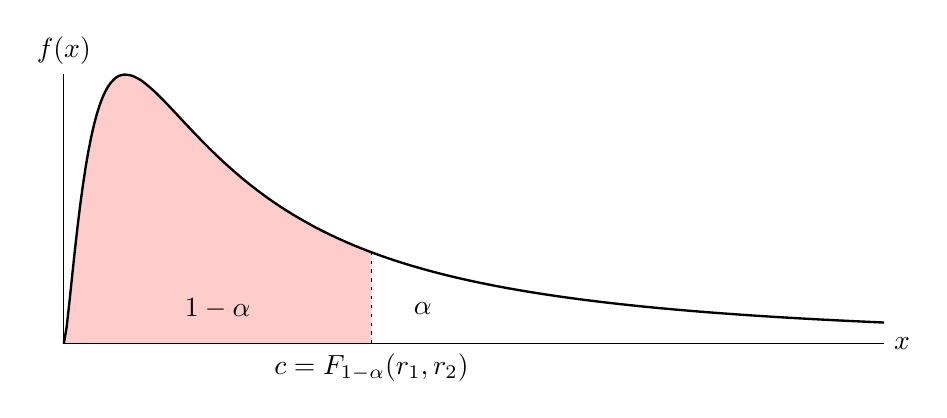
\begin{tikzpicture}[
    declare function={
            gamma(\z)=2.506628274631*sqrt(1/\z)+ 0.20888568*(1/\z)^(1.5)+ 0.00870357*(1/\z)^(2.5)- (174.2106599*(1/\z)^(3.5))/25920- (715.6423511*(1/\z)^(4.5))/1244160)*exp((-ln(1/\z)-1)*\z;
        },
        declare function={
            beta(\x,\y)=gamma(\x)*gamma(\y)/gamma(\x+\y);
        },
    declare function={
        fdst(\x,\a,\b) = 1 / beta(\a/2, \b/2) * (\a/\b)^(\a/2) * \x^(\a/2-1) * (1 + \a/\b*\x)^(-(\a + \b)/2);
    }
]

\begin{axis}[
  no markers, domain=0:4, samples=300,
  axis lines*=left, xlabel=$x$, ylabel=$f(x)$,
  every axis y label/.style={at=(current axis.above origin),anchor=south},
  every axis x label/.style={at=(current axis.right of origin),anchor=west},
  height=5cm, width=12cm,
  xtick=\empty, ytick=\empty,
  enlargelimits=false, clip=false, axis on top,
  grid = major
  ]


\addplot [fill=red!20, draw=none, domain=0:1.5] {fdst(x,5,2)} \closedcycle;
\addplot [very thick,line width=0.3mm] {fdst(x,5,2)};
\draw (0.75,0.075) node[] {$1-\alpha$};
\draw (1.75,0.075) node[] {$\alpha$};
  \node[below] at (axis cs:1.5,0)  {$c=F_{1-\alpha}(r_1,r_2)$}; 
    \draw [very thick, dotted,line width=0.2mm]  (axis cs:1.5,0) -- (axis cs:1.5,0.2);
\end{axis}
\end{tikzpicture}
\end{center}

Para determinar los valores de $F$, correspondientes a areas:

$$1-\alpha = 0.005,0.010,0.025,0.05$$ 

o para determinar probabilidades correspondientes a valores de $c<1$ se usa el teorema siguiente.

\subsubsection{Teorema}
Si:
$$ X\sim F(r_1,r_2) \text{ entonces } \dfrac{1}{X}\sim F(r_2,r_1)$$
esto es:
$$ F_{1-\alpha}(r_1,r_2) = \dfrac{1}{F_{\alpha}(r_2,r_1)} $$

\subsection{Distribución Gamma}
\subsection{Distribución Beta}
\subsection{Distribución de Weibull}
